\documentclass[CJKmath=true,10pt]{MyBook}


\usepackage{graphicx,float}
\usepackage{fontawesome5}
\usepackage[normalem]{ulem}
\usepackage{tikz}
\usetikzlibrary{arrows.meta, calc, patterns}



\newcommand{\cgc}[3][]{
\begin{figure}[H]
\centering
\includegraphics[#1]{#2}
\caption{#3}
\end{figure}}

%设置一些字体
\usepackage{fontspec}
%\setCJKmainfont{Source Han Serif CN}
%[
%	Path=./fonts/hz/,
%	UprightFont = SourceHanSerifCN-Regular,
%	BoldFont = SourceHanSerifCN-Bold,
%	%ItalicFont = SourceHanSerifCN-Regular,
%	%BoldItalicFont = SourceHanSerifCN-Bold
%]
%\setCJKsansfont{Noto Sans CJK SC}
%[
%	Path=./fonts/hz/,
%	UprightFont = NotoSansCJKsc-Regular,
%	BoldFont = NotoSansCJKsc-Bold,
%	%ItalicFont = *-Regular,
%	%BoldItalicFont = *-Bold
%]
%\setCJKmonofont{Noto Sans Mono CJK SC}
%[
%UprightFont = *-Regular,
%BoldFont = *-Bold,
%AutoFakeSlant = 0.2
%]


\begin{document}

%\frontmatter\tableofcontents
\mainmatter
%\setchapterimage{./images/055}
\setchapterimage{./images/bw}
\chapter{传送带专题}
\section{传送带问题一般分析方法}
%\includegraphics{./pics/1.png}
\begin{figure}[H]
\centering
\begin{tikzpicture}[>=Stealth, scale=1]
    % === Left: Conveyor Belt Diagram ===
    \begin{scope}
        \def\R{0.6} % Pulley radius
        \def\L{5.0}   % Distance between pulley centers
        
        % Pulleys
        \filldraw[fill=gray!20] (0,0) circle (\R);
        \filldraw[fill=gray!20] (\L,0) circle (\R);
        \draw[fill=black] (0,0) circle (0.05);
        \draw[fill=black] (\L,0) circle (0.05);
        
        % Belt
        \draw[thick] (0,\R) -- (\L,\R);
        \draw[thick] (0,-\R) -- (\L,-\R);
        
        % Rotation arrow (clockwise on right pulley)
        \draw[->, thick, black] (\L+\R-0.25, \R-0.25) arc (45:-90:0.4);
        
        % Block (placed on left side)
        \coordinate (BlockPos) at (0.4, \R+0.05);
        \draw[fill=blue!30] (BlockPos) rectangle ++(0.8, 0.5);
        \node at ($(BlockPos)+(0.4, 0.25)$) {$m$};
        
        % Velocity vectors
        % v0 (Block)
        \draw[->, thick, red] ($(BlockPos)+(\R/4, 0.05)$) -- ++(1.0, 0) node[right] {$\mu mg$};
        % v (Belt)
        \draw[->, thick, black] (\L/3, \R-0.4) -- ++(1.2, 0) node[right] {$v_0$};
        
        % Labels
        \node[below] at (0,-\R) {$A$};
        \node[below] at (\L,-\R) {$B$};
        
        \node[below, align=center] at (\L/2, -1.0) {传送带足够长};
    \end{scope}

    % === Right: v-t Graph ===
    \begin{scope}[shift={(8,-1)}]
    	\coordinate (O) at (0, 0);
    	\coordinate (TC) at (2, 1.5);
    	\coordinate (T1) at (2, 0);
    	\coordinate (V0) at (0, 1.5);
        
        

        % Axes
        \draw[thick,->] (-0.5, 0) -- (4, 0) node[below] {$t$};
        \draw[thick,->] (0, -0.5) -- (0, 2.5) node[left] {$v$};
        \node[below left] at (O) {$O$};
        
        % Belt velocity v (dashed line)
        \draw[dashed, red, thick] (V0) -- (3.5, 1.5) node[right] {$v_0$};
        \node[left, red] at (0, 1.5) {$v_0$};
        
        % Block velocity behavior: v0 -> v then constant
        % Coordinate definitions

       
        
        
        % Curve
        \draw[blue, thick] (O) -- (TC);
        
        % TC mark
        \draw[dashed] (TC) -- (2, 0) node[below] {$t_1$};
        
        % Fill the area enclosed by O, TC, V0
        \fill[pattern=horizontal lines, pattern color=red] (O) -- (TC) -- (V0) -- cycle;
        \fill[pattern=vertical lines, pattern color=blue] (O) -- (T1) -- (TC) -- cycle;
    \end{scope}
\end{tikzpicture}
\caption{水平红色三角形区域面积表示相对位移,蓝色竖直三角形区域面积表示对地位移。}
\end{figure}
对于水平传送带,只要物块速度比传送带慢,就一定加速。如果传送带慢,物块有初速度并且比传送带快,那么一定减。最终两者会达到共速。
\begin{figure}[H]\centering
    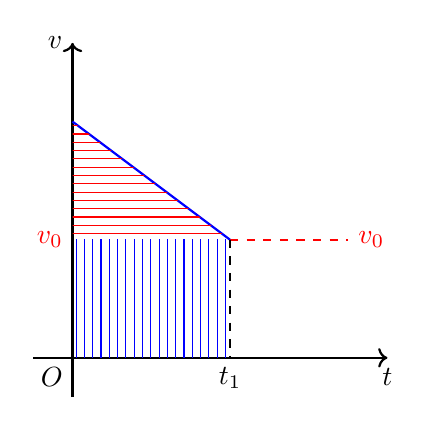
\begin{tikzpicture}
	\coordinate (O) at (0, 0);
	\coordinate (TC) at (2, 1.5);
	\coordinate (T1) at (2, 0);
	\coordinate (V0) at (0, 1.5);
	\coordinate (V1) at (0,3);
	
	
	
	% Axes
	\draw[thick,->] (-0.5, 0) -- (4, 0) node[below] {$t$};
	\draw[thick,->] (0, -0.5) -- (0, 4) node[left] {$v$};
	\node[below left] at (O) {$O$};
	
	% Belt velocity v (dashed line)
	\draw[dashed, red, thick] (TC) -- (3.5, 1.5) node[right] {$v_0$};
	\node[left, red] at (0, 1.5) {$v_0$};
	
	% Block velocity behavior: v0 -> v then constant
	% Coordinate definitions
	
	
	
	
	% Curve
	\draw[blue, thick] (V1) -- (TC);
	
	% TC mark
	\draw[dashed] (TC) -- (2, 0) node[below] {$t_1$};
	
	% Fill the area enclosed by O, TC, V0
	\fill[pattern=horizontal lines, pattern color=red] (V0) -- (TC) -- (V1) -- cycle;
	\fill[pattern=vertical lines, pattern color=blue] (O) -- (T1) -- (TC) -- (V0)--cycle;
\end{tikzpicture}
	\caption{物块比传送带快的情况}
\end{figure}
\begin{itemize}
	\item \textbf{同向}:依据物块初速度和传送带的速度大小\textbf{快减慢加}。
	\item \textbf{反向}则一定减速,减速到0后再加速,然后共速\footnote{此种情况,可以结合竖直上抛运动,两者极为相似,也称\textbf{反上抛}。}。
\end{itemize}

在\textbf{水平}传送带运动中,滑动摩擦力提供的最大加速度$a=\mu g$。如果传送带是匀速的,在共速后,不需要外力,只需要惯性就可以维持物体和传送带一起运动,因此此时的滑动摩擦力一定够用。

如果传送带有加速度,则情况变得复杂了,物体放上传送带时就需要判断最大静摩擦力提供的加速度$\mu g$能否追上传送带的加速度。通常使用$VT图$直接判断,如果$\mu g \ge a_{传送带}$,其实就变成了追击问题;如果小,更简单,永远不能共速,也就是物体一直在传送带上\textbf{打滑}。$a$大$\mu g$小必打滑。

对于水平传送带有加速并且$\mu g \ge a_{传送带}$,在共速后,因为摩擦力可以提供足够的加速度,因此两者一直共速,即物体也和传送带有同样的加速度(物体的加速度不可能超过传送带的加速度)。

对于倾斜传送带,$a_{斜滑}=g\cdot\sin\theta \pm \mu\cdot g\cdot\cos\theta$。如果物体\textbf{相对传送带}沿斜面向上滑,重力在斜面的分量和摩擦力一致,取“$+$”,否则取“$-$”。

视频23分钟要注意。
\end{document}